\section{Theoretical Principles}

\subsection{Deterministic Chaos}

A chaotic system is a dynamical system, which is highly sensitive to its initial conditions. Changing them even by a very small degree leads to a completely different behavior of the system. Thus, a long-term prediction of the behavior is impossible. Nonetheless chaotic systems can be deterministic, meaning that no random or stochastic elements are involved, but they still have unpredictable behavior.

\subsubsection{Bifurcation}

A periodic system usually has a circular trajectory in phase space and is defined by a single sharp frequency. In chaotic systems, this depends on a so called control parameter. By changing this parameter, the system can suddenly be overlaid by a second periodic oscillation with smaller amplitude, so that the resulting system has the double frequency of the initial system. This phenomenon is called a bifurcation. The circle in phase space gets back to its initial point after two cycles and in the spectrum shows two frequencies, the one of the initial system, and one which has half its frequency. By changing the control parameter even more, the system shows more and more of these bifurcations, until it turns into chaos, which means, that an infinite number of subharmonic oscillations overlay the original system. The resulting period of the system is infinite.

\subsubsection{The bifurcation diagram}

If, in the phase space of a chaotic system through bifurcations (as mentioned above), we lay a Poincaré-section, a hyper-section perpendicular to the trajectories, at any point, and we plot those points against the control parameter, we obtain a so called bifurcation diagram, which contains information about when unstable behavior takes place, and how long it lasts.

\begin{figure}[H]
\centering 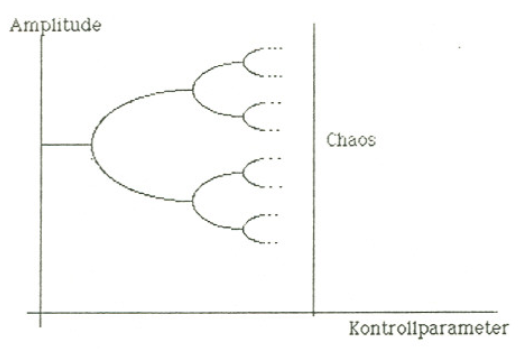
\includegraphics[width=0.8\textwidth]{Bilder/TheoBifDiag.png}
\caption{Representative Example of a Bifurcation Diagram}
\end{figure}

\subsubsection{Feigenbaum-Constants}

Every system, whose path to chaos can be described by bifurcations, underlies a certain universality. This universality is reflected in the Feigenbaum-Constants $\alpha$ and $\delta$.
Let's call $L_n$ the point of the nth bifurcation of our system. The Feigenbaum-Constant $\delta$ is then given by
\begin{equation} \delta = \lim_{n\to \infty} \delta_n = \lim_{n\to \infty}\ \frac{L_{n+1}-L_n}{L_{n+2}-L_{n+1}} = 4.6692016\dots \end{equation} and it has that value for every chaotic system.

\begin{figure}[H]
\begin{minipage}{0.4\textwidth}
The other Feigenbaum-Constant is called $\alpha$. It is defined by \begin{equation} \alpha = \frac{|d_n|}{|d_{n+1}|}=2.502907875\dots\end{equation} The value for $d_n$ is given by the distance from the intersection point of half the amplitude (figure 2 : x=1/2) and the bifurcation diagram to the next fix-point on the diagram. $\alpha$ is the same for any two consecutive bifurcations and any bifurcation diagram.
\end{minipage}
\begin{minipage}{0.6\textwidth}
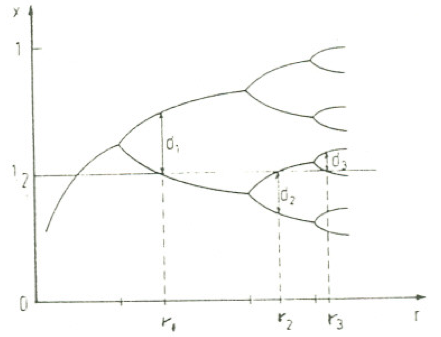
\includegraphics[width=\textwidth]{Bilder/alpha.png}
\caption{How to calculate $\alpha$}
\end{minipage}
\end{figure}

\subsubsection{An example: The Logistic Map}

The logistic map is defined by $$x_{i+1}=r\cdot x_i(1-x_i)$$ with $r$ as the control parameter. It has two fix-points: $$x_0 = 0 \text{\ and \ } x_1 = 1-\frac{1}{r}$$ By changing the control parameter $r$, the logistic map bifurcates. Here is a table describing its behavior in function of $r$:\\

\begin{tabular}{c l}
$0 < r < 1$ & $x_0$ is the only (stable) fix-point\\
$1 < r < 3$ & $x_0$ is unstable and $x_1$ is a stable fix-point\\
$3 < r < 4$ & there is no more stable fix-point\\
$4 < r$ & the system is completely chaotic
\end{tabular}

\begin{figure}[H]
\centering 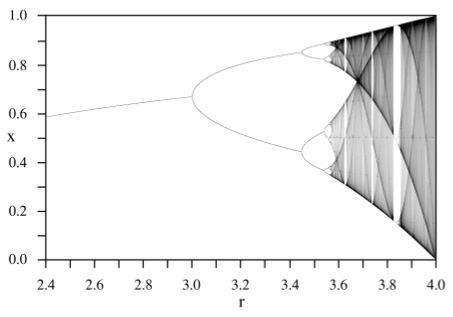
\includegraphics[width=0.8\textwidth]{Bilder/logmap.png}
\caption{Bifurcation-Diagram of the Logistic Map}
\label{bifurcation-diagram-of-the-logistic-map}
\end{figure}

\subsubsection{Periodic windows}

It is possible in a chaotic system, that by changing the control parameter, at one point the system starts being periodic again with stable fix-points. By even further increasing the control parameter, those \emph{windows} start bifurcating again until the system becomes chaotic again. For an example of a window, see fig. \ref{bifurcation-diagram-of-the-logistic-map} of the logistic map, with $r$ around 3.83.


\subsection{The linear oscillating circuit}
\begin{figure}[H]
\begin{minipage}{0.5\textwidth}
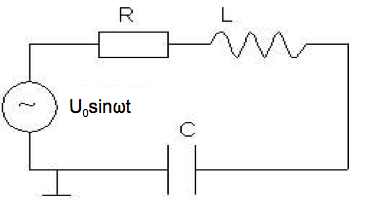
\includegraphics[width=\textwidth]{Bilder/lincirc.png}
\caption{Diagram of a RLC-circuit}
\end{minipage}
\begin{minipage}{0.5\textwidth}
With Kirchhoff's law we get the relation \begin{eqnarray*}  
U_{ext} &=& U_0\cdot\sin\omega t \\
&=& U_L + U_R + U_C\\
&=& L\cdot \dot I + R\cdot I + Q/C
\end{eqnarray*}
With the relation $I = \dot Q$ we obtain the differential equation:
$$ L\ddot Q + R \dot Q + \frac{1}{C}Q = U_0\cdot\sin \omega t $$
\end{minipage}
\end{figure}

Using the ansatz $Q(t) = Q_0 \cdot\cos(\omega t)$ we get:

$$Q(t) = \frac{U_{ext}}{-\omega^2L+i\omega R + 1/C}$$

and from this follows, that

$$U(\omega) = \frac{ \frac{U_0}{LC} }{ \sqrt{ (\frac{1}{LC} - \omega^2 )^2+ (\frac{R}{L}\omega)^2}}$$

We use this formula to fit the data of the linear oscillating circle:

\begin{equation} U(\omega) = \sqrt{\frac{A^2}{(B^2-4\pi^2f^2)^2 + (2\pi Cf)^2}} \end{equation}

with  $A=\frac{U_0}{LC}$ ,  $B=\frac{1}{\sqrt{LC}}$ ,  $C=\frac{R}{L}$

\subsection{The nonlinear oscillating circuit}
\begin{figure}[H]
\begin{minipage}{0.5\textwidth}
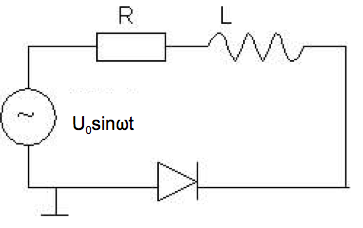
\includegraphics[width=\textwidth]{Bilder/nlcirc.png}
\caption{Diagram of a RLC-circuit}
\end{minipage}
\begin{minipage}{0.5\textwidth}
In order to build a nonlinear oscillating circuit, we use a diode instead of a capacitor.  With the conditions
$$U_{ext} = L\dot I + R\dot I + U_{diode}$$
$$I_{ext}-I_{diode} = \dot Q = C(U)\dot U$$
we get the differential equation for the circuit:
\end{minipage}
\end{figure}

\begin{equation} 
\ddot Q + \left(\frac{R}{L} + \frac{1}{C(Q)} \frac{\partial I_{diode}}{\partial U}\right) \dot Q + \frac{1}{L} \left(RI_{diode}+U \right) = U_{ext}
\end{equation}

The differential equation can easily be identified as a driven damped oscillator with a nonlinear damping coefficient
\begin{equation}
 a \left( Q \right) = \left(\frac{R}{L} + \frac{1}{C(Q)} \frac{\partial I_{diode}}{\partial U}\right)
\end{equation}
 as well as a nonlinear restoring force
\begin{equation}
 f \left( Q \right) = \frac{1}{L}(RI_{diode}+U)
\end{equation}

The charges on the diode can be obtained by integrating over the capacitance:
\begin{equation}
 Q \left( U \right) = \int_0^U C \left( U' \right) dU'
\end{equation}

Nonlinear diodes are usually build out of semiconductor material, which is doped to create a p-n-junction. On one side of this junction, the p-side, lattice atoms (usually silicon with 4 valence electrons) are replaced with atoms having fewer valence electrons. Thus an electron would result in lower energetic state and this atom is considered as "missing" one electron. The free spot for the electron is called a hole. On the other side, the n-type material is produced by doping with materials having a higher valence electron count. This leads to an excess in electrons. Directly at the junction, electrons and junctions interchange, creating an electric field in doing so, which blocks further migration.

When a negative voltage is applied to such a single p-n-combination (called a semiconductor diode), it increases the electric field and no current flows. This is called the blocking direction of the diode. Its capacitance can be described by
\begin{equation}
 C \left( V \right) = \frac{C_0}{\sqrt{1-V/\phi}}
\end{equation}

Switching to a positive voltage, for some short time it is compensated, leading to the capacitance
\begin{equation}
 C \left( V \right) = C_0 \cdot e^{\frac{V}{\phi}}
\end{equation}
before the junction-field is flooded and current sets in.

This time-lag leads to an interesting behavior. If in such a circuit, the amplitude of the driving voltage is increased, the system bifurcates until its trajectories are completely chaotic. 

